\section{Field Study}
\label{sec:field-study}


	The field study took place during the first two weeks of March, from 3/3/2015 to 3/15/2015 in a faculty building of Ludwig-Maximilians-University Munich. Data was collected on 14 consecutive days and personal semi-structured interviews were carried out on five working days during the same two weeks. A total of 118 interactions were registered with the application installed on the public display and 58 survey responses were recorded.

	The goal of this study was to validate the previous thoughts, get better insights into our research questions, and to see how users respond to questionnaires being conducted on displays in the public.




\subsection{Research Questions}

	% MOTIVATE: explain why we make this field study, explain what we hope to expect. what are our assumptions. what did we expect from the questionnaires, what did we expect from the interviews?

	One of the main reasons why we performed this field study was to get a better understanding of our assumptions and hypotheses. Especially since there is often a discrepancy between what one assumes and what can actually be observed in real world. This phenomena has already been stated in the publication by Ojala and Kostakos in 2011: ``Introduction A common criticism targeted at many studies on interactive public displays is that their evaluation usually takes place in non-realistic lab environments, and for short periods of time. Thus, a long-term real- world deployment could be a more appropriate evaluation.''\cite{Ojala2011}.

	% Why did we bother to do this study?
		% to find out if our results and predictions validate in the field

	% What do we assume
	% What do we want to know
		% which variables are there, how do we expect them to change?

	The assumption we made for the development of our first research prototype of the PDSurvey platform is that we can simplify the conduction and deployment of surveys to large public display networks. Since this is a rather large claim, we broke down the hypothesis to multiple more fine-grained statements. The claim, whether the PDSurvey platform facilitates the conduction of large-scale surveys in public, will be evaluated in the following chapter (see chapter \ref{sec:expert-interview}). 

	What we will evaluate in the scope of this thesis, are the following research questions:

	\begin{enumerate}
	\item Which question types are best suited for questionnaires carried out in public? How should a survey be constructed to take best advantage of the PDSurvey platform? (quantitative vs. qualitative)

	\item Which channels are most suited for completing surveys (on a digital platform) in public?
		% The first step was to ask ourselves the question, which channel is suited for gathering responses from the audience. ...

		% We already had an application running on a public display in a faculty building which attracted lots of regular and new users. Our interest was how we could best integrate questionnaires on and after the application itself (a balloon shooter game).
	\item (assessed between the lines) What motivated our users to fill out surveys?
	\end{enumerate}


	Research questions which would go beyond the scope of this thesis, and might serve as follow-up questions for further research are gathered here:

	\begin{itemize}
	\item In which situations is the user most willing to answer surveys on public displays?
	\item (not really copious): how many questions are acceptable, the attention span would be of great interest
	\item (not really copious): how the users noticed / perceived the survey
	\item (Not treated): where to position the survey on screen. As stated in a paper by J\"org M\"uller ... TODO reference it TODO ..., the best position on large public displays is directly in the center (not at the bottom, not at the top, close to the center). The larger the screen is, the more relevant a centric positioning will get.
	\item (Not treated): The influence of the environment on which question types are suited, how personal the questions can get, how much privacy the display should offer (the smaller the display, the more private the context seems)
	\item (Not treated): How can we best break down a standardized survey with 10+ questions and spread a subset of the questions across multiple users?
	\end{itemize}

	In addition to these questions we were also interested in user stories, in the feedback real-world users gave us in regards to answering surveys on screens in the public. For this reason we also conducted semi-structured interviews in parallel to the quantitative evaluation of the PDSurvey platform.




\subsection{Study Setup}

	Both quantitative and qualitative data was gathered as part of the field study. Quantitative data was obtained through the PDSurvey system and qualitative data was collected through semi-structured interviews. To facilitate comparison between quantitative and qualitative data some quantitative questions were asked redundantly at the end of the semi-structured interview, in order to make the mapping of participant to semi-structured interview easier.

	% \subsubsection{Design}

	% 	\begin{enumerate}
	% 	\item provide an overview of the overall structure of your experiment. 
	% 	\item what were the independent variables in the study? what were the factors that I manipulated? >> none! 
	% 	\item how many conditions were there: ... i would say none, since I didn't vary any parameters
	% 	\item describe what was measured, what were the dependent variables?
	% 	\item >>> I would actually say, that I didn't carry out any experiment, I only made an observation with evaluation. I didn't vary any parameters, I only configured a study setup and observed + interviewed the participants
	% 	\end{enumerate}


	\subsubsection{Participants}
		% provide the necessary information about the people who took part in your experiment

		The questionnaires were filled out by a random number of people with different backgrounds. What they had in common was their affiliation to LMU Munich, either being a student, staff or otherwise related (parents, pensioner, industry partner).

		In regards to the field study all participants can be differentiated in three study groups: participants who approached the display by themselves (and were observed doing so), people passing by the display (noticing the display, however not approaching it) and the last group of people (simple passing by, not having any intention to approach the display).

		+ STATE THE NUMBERS

		In total 

		\begin{enumerate}
		\item give details on how many participants you used
		\item how many took part in which condition
		\item include information about demographic values (age, gender)
		\item also deliver brief details on how you obtained the participants: they didn't get any reward for participating. XX were passerby, XX participated in the game from their own motivation.
		\item describe the population of my participants. what was their background?
		\item  Before starting the interviews the people participating and passing by were asked whether they noticed the option to fill out a survey, and XX out of XX didn't notice the option. 
		\item think about which information is relevant. for me the devices they possess might be of relevance. people not possessing a smartphone or tablet, might be less willing to use these devices.  
		\end{enumerate}

	\subsubsection{Apparatus}
		% give details of any equipment used, including thinkgs like questionnaires and other tests

		The apparatus consisted of a XXX-inch TV screen, a Samsung Galaxy tablet, two questionnaires (one for participants, one for passerby), a voice-recorder (smartphone), and the client of the PDSurvey platform installed on the TV screen and on the tablet.

		+ SHOW A PHOTO OF THE STUDY SETUP

		Our object of investigation was theTV screen with touch support, running an interactive \textit{Balloon Shooter} game. After completing the game users were asked to complete a questionnaire via one of the four offered feedback channels. 

		Each user had the opportunity to respond directly on the TV display (1), to the right on a tablet (2), via their smartphone (3) or via email (4). The first option was embedded directly into the Balloon Shooter game, offering a consistent UI and the most direct feedback channel (see screenshot TODO \ref{screenshot:5-options}). Choosing the tablet option users were prompted to move to the right and to answer five questions on the tablet (see screenshot \ref{screenshot:5-tablet}). The Galaxy Samsung Tab 10.1 was displaying the responsive frontend of PDClient, being enclosed in a Android Kiosk App, namely KioWare Lite\footnote{http://www.kioware.com/android.aspx}. Choosing the option to use a smartphone prompted the user to either scan a QR code or to access a URL (see figure \ref{screenshot:5-mobile}). The last option consisted of an input field embedded into the Balloon Shooter game on the TV screen, asking the user to enter their email address. The address was logged to a txt-file on the Windows machine and processed by a Python script, which sent a ... 

		% reference and embed all four screenshots for every feedback channel, show with what the user was confronted with.

		% maybe also show a flow of actions, but not sure if this is needed, when the user can also simply read the previous paragraph.


		% + state how we motivated the users to participate: only 5 questions, results are for a MA thesis

		% + give more information about the balloon shooter game.


		For the evaluation in the field study itself a self-made questionnaire was used, since the focus was on finding which channels and question types are best suited in general for being used on public display. This was the reason why we did not use any of the standardized questionnaires mentioned in section \ref{sec:questionnaires}. The questionnaires used can be found in the Appendix.

		More information regarding the Balloon Shooter game can be found here XXXXX. 
		The main application installed on the public display was a game called \textit{Balloon Shooter} developed and run by Jiamin Shi, a PhD student at the Group for Media Informatics at LMU Munich. It was first installed on January 7th 2015 and has been running in different versions since then. Public audience was already used to it for roughly two months and adapted to it well.

		% + ask Jiamin, whether and which screenshots of the game I am allowed to post?





	\subsubsection{Procedure}
		% tell the reader how the study was carried out in practice
		= equivalent to the method section?



		\begin{enumerate}
		\item How I introduced the scenario to the passerby. Imagine you are in a shopping mall or at an airport using one of those large displays to find some information. In the end you get asked to answer a short questionnaire. (How would you react to it? And to the more qualified students with the right background I also asked how they would feel when getting asked quantitative or qualitative data. / KW-student) 
		\end{enumerate}


	\subsubsection{Location}

	Faculty building for computer science, ethnology, political science, japanologie and physics. m,m

	The study setup was in the entrance hall of the university building, .

	+ SHOW A DIAGRAM OF THE User paths inside the entrance hall.


	\subsubsection{Limitations}

	\begin{enumerate}
	\item the tablet was always on, it was possible to approach the tablet directly without having the option to participate in the survey via smartphone or email. 
	\item the novelty effect played a role for the first part of the evaluation. It was striking to see a response rate of 50 percent. If we exclude all participants who directly accessed the tablet and skipped the appeal to use one of the four options, there was still a response rate of 10 percent.
	\end{enumerate}



\subsection{Conditions}

	Feedback channel: 
	\begin{enumerate}
	\item on public display
	\item on tablet, next to the large TV display
	\item via smartphone: 
	\item via email, from home:
	\end{enumerate}


\subsection{Methodology}



\subsection{Quantitative Results}

	\begin{enumerate}
	\item For a good SAMPLE of how to list the basic population (x male, y female) of the survey, have a look at paper number 25 from the Appendix. (WIP)
	\item describe the results from the evaluation
	\item e.g. 1) prefered feedback channel, 2) number of acceptable answers, 3) preferred setting
	\item say which implications this gives for the PDSurvey research platform
	\end{enumerate}

	\begin{enumerate}
	\item Quantitative: pure facts
	\item Qualitative: a combination of facts + evaluation
	\end{enumerate}


	Our primary goal was to find out which channel the users preferred, the questions themselves played a secondary role. The survey displayed on all four channels contained the same five questions. 

	\begin{itemize}
	\item How often have you used this display before? [number]
	\item How likely is it that you will use this display in the future again? [5-point Likert scale]
	\item Which devices do you possess or use regularly? [multiple choice with 5 check boxes]
	\item In which area do you study / work? [text field]
	\item What was your motivation for approaching and using this display? [text field]
	\end{itemize}

	In order to also get first insights into how well certain question types are suited for surveys in public, where a short completion time is crucial, we varied between the following question types and kept them in the same order: numerical question, Likert scale (single click), multiple choice (based on check boxes) and two text fields for an undefinied length of the response. To increase the motivation for participation we stated that the questionnaire consists of five questions, will only take one minute to complete and is for the Master's thesis of student at LMU Munich (see figure \ref{fig:5-pdclient-intro}).
	As proven by Richard Ryan in his self-determination theory\cite{ryan2000self}\footnote{http://www.selfdeterminationtheory.org/}, this additional intrinsic motivation increased the participation and acceptance rate of the public survey additionally. 

	\begin{figure}
	    \begin{center}
	        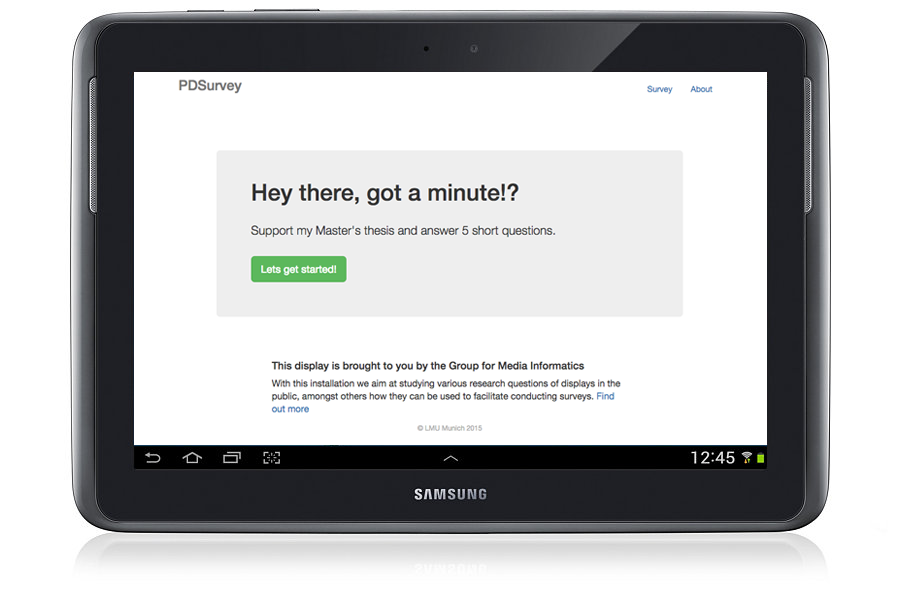
\includegraphics[width=.7\columnwidth]{img/5_field-study/pdclient-startscreen.png}
	    \end{center}
	 \caption{PDClient: Motivating users to participate in a short questionnaire}
	 \label{fig:5-pdclient-intro}
	\end{figure}

	The first question (numeric) was completed in all surveys. 

	To find out more about the motive we carried out semi-structured interviews on location.


\subsection{Qualitative Results}

	%% Evaluation based on Grounded Theory
	% for systematic evaluation of qualitative data (interview transcripts)
	% while having the goal of generating a theory
	% > datengestützte Theoriebildung = auf Empirie bezogene Bildung von Hypothesen / Theorien


\subsection{Discussion AND/OR Summary}

	% 1) Start with a few sentences that summarize the most important results (+ see \url{http://www.ldeo.columbia.edu/~martins/sen_sem/thesis_org.html}).

	\begin{enumerate}
	\item (summarize the expert interviews)
	\item summarize the quantitative results
	\item summarize the qualitative results 
	\item TODO: think about what my evaluation has to do with my platform. make sure that this link is clear! Make this link clear in the following summary.
	\end{enumerate}

	% 2) Now allowing room for interpretation and personal opinions:

	\begin{enumerate}
	\item \textbf{questions in the public} / questionnaires on public displays are best suited for quantitative surveys. Users want a short interaction time, not having to think much about their answers and for roughly XXXXX percent of the participants it holds true, that they do not like being observed while making responses in public.

	\item From this observation, the implication for the \textbf{question types} can be derived: question types ideally with a single-click interaction are preferred (e.g. Likert scale, multiple choice with all options given, yes/no-questions). Then followed by numeric, dropdown and multiple choice questions with an open end. For these question types the user has to think a little bit more, he has to assess more precisely in order to make his response. One example stated by a participant, in regards to the numeric question `How often have you used this display before?', was that ``It would be great if you had the possibility to choose from a predefined range, because typing is not always optimal. I would prefer if areas would be given instead of oneself having to think about the exact number.'' Last, being no big surprise, are text fields combined with open-ended questions. As a take away for text fields: wherever possible rephrase the question so that you can respond to it as short as possible.

	\item and in regards to the \textbf{feedback channel}, no clear recommendation can be made. All offered feedback channels were present in the evaluation and during the semi-structured interviews for each channel a good reason was given. What can be said that the crowd usually distinguishes into three groups. The first (and slightly larger) group preferring the option of \textit{direct response}. They are not as considerate about answering questions in public and their privacy aspect. For them it is more important to complete the survey as quick as possible and not having to think about it later, as long as nothing too private or personal gets asked. One person said ``If something too private would be asked, I would simply abort and go away from the display''. The second group is more privacy concerned, often older of age, or actually wanting to take the time to think about all of their responses in depth in order to give high-quality responses. This group prefers to take the questionnaire away from the public setting into their home. The last group choose the feedback channel purely based on their \textit{habit} and what they are accustomed to. Two ladies in their mid-twenties responded immediately ``on my smartphone, because I am most used to it''.

	\item and regarding the \textbf{display size}: the smaller the display, the safer and more private they feel. An exception to this finding could be old people. Once people become short-sighted or more insecure and unconfident with using new devices, they prefer having a large input surface.

	\end{enumerate}



	% 3) Restate and make sure, what my evaluation has to do with my platform. make sure that this link is clear!



